% Op icon: wedge — right-triangle front face, tall right-side face, slanted ramp face.
% Depth offset (3,5) is deliberately NOT parallel to the front hypotenuse (slope 1)
% and points away from the front face's interior on both faces it's applied to —
% picking (4,4) here previously made the ramp face degenerate (collinear with the
% hypotenuse) and made the side face overlap the front face. Verified by rendering.
\documentclass[tikz,border=2mm]{standalone}
\usetikzlibrary{arrows.meta,calc,shapes.geometric}
\begin{document}
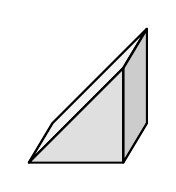
\begin{tikzpicture}[line width=1.3pt, line cap=round, line join=round, >=Stealth, x=1mm,y=1mm]
  \coordinate (A) at (-6,-8);
  \coordinate (B) at (6,-8);
  \coordinate (D) at (6,4);
  \coordinate (A2) at (-3,-3);
  \coordinate (B2) at (9,-3);
  \coordinate (D2) at (9,9);
  \draw[thick, fill=gray!10] (A) -- (D) -- (D2) -- (A2) -- cycle;
  \draw[thick, fill=gray!40] (B) -- (D) -- (D2) -- (B2) -- cycle;
  \draw[thick, fill=gray!25] (A) -- (B) -- (D) -- cycle;
\end{tikzpicture}
\end{document}
